\documentclass{article}
\usepackage{graphicx}
\usepackage[utf8]{inputenc}
\graphicspath{ {./pictures} }

\title{Rozdział}
\author{Mikołaj Durkot}
\date{November 2022}

\begin{document}
\maketitle

\[E=mc^2\]

\begin{center}
   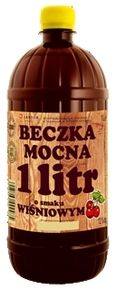
\includegraphics{Pictures/napuj_boguw.jpg} 
    \label{fig:zdjecie}
\end{center}

\begin{table}[]
\resizebox{\textwidth}{!}{%
\begin{tabular}{|c|c|c|c|c|}
\hline
1 & 2 & 3  & 4  & 5  \\ \hline
2 & 4 & 6  & 8  & 10 \\ \hline
3 & 6 & 9  & 12 & 15 \\ \hline
\end{tabular}%
}
\label{fig:tabela}
\end{table}

\section{numerowana:}
\begin{enumerate}
    \item raz
    \item dwa
    \item trzy
\end{enumerate}


\section{nienumerowana:}
\begin{itemize}
    \item cztery
    \item sześć
\end{itemize}

\section*{lateks}

\setlength{\parindent}{20pt}

\section*{paragrafs}
\textbf{piwo} to moje paliwo

\textbf{jabol} tez lubie.

\noindent\textbf{nie wiem co napisac}. pisze cos bla bla dobre spegety zjadlem

blabla \emph{jaja} 
blablablabla
gra

\textit{no dzien dobry \emph{ogulem} 
o wlasnie}

\textbf{kabab \underline{z kapusniakiem} 
ja nie komar
ja major.}
\section*{zdjecie}
\pageref{fig:zdjecie}
\section*{tabela}
\pageref{fig:tabela}
\end{document}